% =====================================================================
%  Whether One Step Is Enough Is Not Determined by the Data
%  -- ICLR 2027 submission draft (anonymous)
%  编译: pdflatex -> bibtex -> pdflatex -> pdflatex（推荐用 code/analysis/build_paper.py）
%  数值宏全部来自 numbers_theory.tex，由 code/analysis/make_theory_macros.py
%  从 logs/*.json 与 results/*.json 自动生成，勿手改。
%  （旧版的 numbers.tex 与其流水线已归档到 _archive_20260916/。）
% =====================================================================
\documentclass{article}
\usepackage{iclr2027_conference,times}
% hypertexnames=false prevents duplicate PDF anchors when floats are deferred across
% the main-text/appendix boundary by the conference style.
\usepackage[hidelinks,hypertexnames=false]{hyperref}
\usepackage{url}
\usepackage{amsmath,amssymb,booktabs,multirow}
\usepackage{amsthm}
\usepackage{graphicx}
\usepackage{xcolor}
\usepackage{adjustbox}
% 表格统一缩小到栏宽。第三轮重写后论文只有 2 张手写的小表，
% 不再经过 tables/*_body.tex（那批旧表在 _archive_20260916/ 里）。
\newcommand{\tblstyle}[1]{%
  \begin{adjustbox}{max width=\columnwidth}%
  \footnotesize\setlength{\tabcolsep}{4pt}%
  #1%
  \end{adjustbox}}
\usepackage{algorithm}
\usepackage{algorithmic}

% 正文所有实验数字都来自这里；由 code/analysis/make_theory_macros.py 生成。
% （旧版的 numbers.tex 已不被引用，见 _archive_20260916/。）
% 自动生成，勿手改。由 code/analysis/make_theory_macros.py 从 logs/ 与 results/ 读出。
% 每个宏的来源都写在行末注释里。
\newcommand{\ImpRhoZero}{0.05006}  % verify_impossibility: curve.rho_hat[0] (alpha=0.00)
\newcommand{\ImpRhoQuarter}{0.1054}  % verify_impossibility: curve.rho_hat[1] (alpha=0.25)
\newcommand{\ImpRhoHalf}{0.2854}  % verify_impossibility: curve.rho_hat[2] (alpha=0.50)
\newcommand{\ImpRhoThreeQ}{0.5747}  % verify_impossibility: curve.rho_hat[3] (alpha=0.75)
\newcommand{\ImpRhoOne}{0.9766}  % verify_impossibility: curve.rho_hat[4] (alpha=1.00)
\newcommand{\ImpAlphaSweep}{0.9265}  % rho_hat(1) - rho_hat(0)
\newcommand{\ImpDDev}{0.002993}  % deviations.max_d_dev
\newcommand{\ImpLamDev}{0.00028}  % deviations.max_lam_dev
\newcommand{\ImpPredMad}{0.007836}  % deviations.pred_mad
\newcommand{\ImpKnnK}{20}  % params.KNN_K[0]
\newcommand{\ImpSeeds}{3}  % params.seeds
\newcommand{\ImpAlphas}{5}  % params.alphas
\newcommand{\ImpC}{4}  % params.C
\newcommand{\ImpK}{8}  % params.K
\newcommand{\ImpVerdict}{PASS}  % verdict
\newcommand{\MinimaxConst}{0.5}  % verify_minimax: constant_baseline.worst
\newcommand{\MinimaxConstAt}{0.5}  % constant_baseline.c_star
\newcommand{\MinimaxDevD}{0.005295}  % stat_rel_dev.D
\newcommand{\MinimaxPD}{0.352}  % stat_anova.D.p
\newcommand{\MinimaxFD}{1.17}  % stat_anova.D.F
\newcommand{\MinimaxCVD}{0.00564}  % stat_cv.D
\newcommand{\MinimaxDevLam}{0.003768}  % stat_rel_dev.Lambda
\newcommand{\MinimaxPLam}{0.86}  % stat_anova.Lambda.p
\newcommand{\MinimaxFLam}{0.322}  % stat_anova.Lambda.F
\newcommand{\MinimaxCVLam}{0.00606}  % stat_cv.Lambda
\newcommand{\MinimaxDevKCH}{0.01242}  % stat_rel_dev.K_CH
\newcommand{\MinimaxPKCH}{0.349}  % stat_anova.K_CH.p
\newcommand{\MinimaxFKCH}{1.18}  % stat_anova.K_CH.F
\newcommand{\MinimaxCVKCH}{0.0147}  % stat_cv.K_CH
\newcommand{\MinimaxDevNNDist}{0.004271}  % stat_rel_dev.nn_dist
\newcommand{\MinimaxPNNDist}{0.627}  % stat_anova.nn_dist.p
\newcommand{\MinimaxFNNDist}{0.66}  % stat_anova.nn_dist.F
\newcommand{\MinimaxCVNNDist}{0.00776}  % stat_cv.nn_dist
\newcommand{\MinimaxDevSep}{0.06374}  % stat_rel_dev.sep8
\newcommand{\MinimaxPSep}{0.466}  % stat_anova.sep8.p
\newcommand{\MinimaxFSep}{0.931}  % stat_anova.sep8.F
\newcommand{\MinimaxCVSep}{0.081}  % stat_cv.sep8
\newcommand{\MinimaxDevKurt}{0.003709}  % stat_rel_dev.kurtosis
\newcommand{\MinimaxPKurt}{0.573}  % stat_anova.kurtosis.p
\newcommand{\MinimaxFKurt}{0.745}  % stat_anova.kurtosis.F
\newcommand{\MinimaxCVKurt}{0.0039}  % stat_cv.kurtosis
\newcommand{\MinimaxDevTrVar}{0.004113}  % stat_rel_dev.trVar_marginal
\newcommand{\MinimaxPTrVar}{0.218}  % stat_anova.trVar_marginal.p
\newcommand{\MinimaxFTrVar}{1.58}  % stat_anova.trVar_marginal.F
\newcommand{\MinimaxCVTrVar}{0.00577}  % stat_cv.trVar_marginal
\newcommand{\MinimaxDevMax}{0.06374}  % max over stat_rel_dev
\newcommand{\MinimaxPAlpha}{0.05}  % params.ALPHA_P (ANOVA level)
\newcommand{\MinimaxPairedMad}{0.01405}  % paired_rho_mad
\newcommand{\MinimaxRiskRatio}{35.58}  % risk_ratio
\newcommand{\MinimaxNStats}{7}  % number of data-only statistics tested
\newcommand{\LadderSnrDFirst}{0.486}  % sample_size_ladder[1000].D.snr
\newcommand{\LadderSnrDLast}{2.95}  % sample_size_ladder[16000].D.snr
\newcommand{\LadderSnrSepFirst}{0.912}  % sample_size_ladder[1000].sep8.snr
\newcommand{\LadderSnrSepLast}{0.693}  % sample_size_ladder[16000].sep8.snr
\newcommand{\LadderSnrKCHFirst}{0.816}  % sample_size_ladder[1000].K_CH.snr
\newcommand{\LadderSnrKCHLast}{0.816}  % sample_size_ladder[16000].K_CH.snr
\newcommand{\LadderSnrNNDistFirst}{0.777}  % sample_size_ladder[1000].nn_dist.snr
\newcommand{\LadderSnrNNDistLast}{0.297}  % sample_size_ladder[16000].nn_dist.snr
\newcommand{\LadderSnrKurtFirst}{0.0718}  % sample_size_ladder[1000].kurtosis.snr
\newcommand{\LadderSnrKurtLast}{1.87}  % sample_size_ladder[16000].kurtosis.snr
\newcommand{\LadderNFirst}{1000}  % smallest n
\newcommand{\LadderNLast}{16000}  % largest n
\newcommand{\LadderWorstAbsDiff}{0.003}  % max over n and over {D,nn_dist,kurtosis} of |S(1)-S(0)|
\newcommand{\LadderAbsMax}{0.01}  % params.ABS_MAX
\newcommand{\MinimaxVerdict}{PASS}  % verdict
\newcommand{\CondDIndep}{0.9116}  % verify_conditional_theory: D.independent
\newcommand{\CondDTrans}{0.9116}  % D.transport
\newcommand{\CondDDiff}{\ensuremath{6.661\times 10^{-16}}}  % D.abs_diff
\newcommand{\CondRhoInd}{0.02722}  % knn_sweep[k=30].rho_ind
\newcommand{\CondRhoDet}{0.8776}  % knn_sweep[k=30].rho_det
\newcommand{\CondContrast}{32.24}  % best_contrast.ratio
\newcommand{\CondKnnK}{30}  % best_contrast.k
\newcommand{\CondKTimesOne}{1.002}  % knn_sweep[k=1].k_times_rho_ind
\newcommand{\CondRhoIndOne}{1.002}  % knn_sweep[k=1].rho_ind
\newcommand{\CondKTimesTwo}{0.9775}  % knn_sweep[k=2].k_times_rho_ind
\newcommand{\CondRhoIndTwo}{0.4888}  % knn_sweep[k=2].rho_ind
\newcommand{\CondKTimesFive}{0.9369}  % knn_sweep[k=5].k_times_rho_ind
\newcommand{\CondRhoIndFive}{0.1874}  % knn_sweep[k=5].rho_ind
\newcommand{\CondKTimesTen}{0.8885}  % knn_sweep[k=10].k_times_rho_ind
\newcommand{\CondRhoIndTen}{0.08885}  % knn_sweep[k=10].rho_ind
\newcommand{\CondKTimesTwenty}{0.8257}  % knn_sweep[k=20].k_times_rho_ind
\newcommand{\CondRhoIndTwenty}{0.04129}  % knn_sweep[k=20].rho_ind
\newcommand{\CondKTimesThirty}{0.8165}  % knn_sweep[k=30].k_times_rho_ind
\newcommand{\CondRhoIndThirty}{0.02722}  % knn_sweep[k=30].rho_ind
\newcommand{\CondVerdict}{PASS}  % verdict
\newcommand{\MSEndpointErr}{\ensuremath{8.882\times 10^{-16}}}  % verify_multistep_theory: endpoint_identity_max_err
\newcommand{\MSVarOne}{\ensuremath{3.592\times 10^{-32}}}  % one_step_spread
\newcommand{\MSRhoOne}{\ensuremath{3.936\times 10^{-33}}}  % sweep[N=1].rho
\newcommand{\MSCovOne}{0}  % sweep[N=1].modes_covered
\newcommand{\MSRhoTwo}{0.5907}  % sweep[N=2].rho
\newcommand{\MSCovTwo}{8}  % sweep[N=2].modes_covered
\newcommand{\MSRhoFour}{0.8573}  % sweep[N=4].rho
\newcommand{\MSCovFour}{8}  % sweep[N=4].modes_covered
\newcommand{\MSRhoEight}{0.9233}  % sweep[N=8].rho
\newcommand{\MSCovEight}{8}  % sweep[N=8].modes_covered
\newcommand{\MSRhoSixteen}{0.9612}  % sweep[N=16].rho
\newcommand{\MSCovSixteen}{8}  % sweep[N=16].modes_covered
\newcommand{\MSRhoThirtyTwo}{0.9815}  % sweep[N=32].rho
\newcommand{\MSCovThirtyTwo}{8}  % sweep[N=32].modes_covered
\newcommand{\MSRhoSixtyFour}{0.992}  % sweep[N=64].rho
\newcommand{\MSCovSixtyFour}{8}  % sweep[N=64].modes_covered
\newcommand{\MSRhoOneTwentyEight}{0.9974}  % sweep[N=128].rho
\newcommand{\MSCovOneTwentyEight}{8}  % sweep[N=128].modes_covered
\newcommand{\MSRhoTwoFiftySix}{1}  % sweep[N=256].rho
\newcommand{\MSCovTwoFiftySix}{8}  % sweep[N=256].modes_covered
\newcommand{\MSVerdict}{PASS}  % verdict
\newcommand{\MMIndepOneRho}{0.00669}  % method_map: summary.cfm_indep@1.rho
\newcommand{\MMIndepOneStd}{0.00159}  % summary.cfm_indep@1.rho_std
\newcommand{\MMIndepOneCov}{0.05}  % summary.cfm_indep@1.coverage
\newcommand{\MMIndepManyRho}{0.9646}  % method_map: summary.cfm_indep@32.rho
\newcommand{\MMIndepManyStd}{0.009531}  % summary.cfm_indep@32.rho_std
\newcommand{\MMIndepManyCov}{8}  % summary.cfm_indep@32.coverage
\newcommand{\MMOtOneRho}{0.8949}  % method_map: summary.cfm_ot@1.rho
\newcommand{\MMOtOneStd}{0.0164}  % summary.cfm_ot@1.rho_std
\newcommand{\MMOtOneCov}{8}  % summary.cfm_ot@1.coverage
\newcommand{\MMReflowOneRho}{0.9631}  % method_map: summary.reflow@1.rho
\newcommand{\MMReflowOneStd}{0.008115}  % summary.reflow@1.rho_std
\newcommand{\MMReflowOneCov}{8}  % summary.reflow@1.coverage
\newcommand{\MMDistillOneRho}{0.9654}  % method_map: summary.distill@1.rho
\newcommand{\MMDistillOneStd}{0.01008}  % summary.distill@1.rho_std
\newcommand{\MMDistillOneCov}{8}  % summary.distill@1.coverage
\newcommand{\MMLtwoOneRho}{\ensuremath{9.815\times 10^{-5}}}  % method_map: summary.onestep_l2@1.rho
\newcommand{\MMLtwoOneStd}{\ensuremath{8.811\times 10^{-5}}}  % summary.onestep_l2@1.rho_std
\newcommand{\MMLtwoOneCov}{0}  % summary.onestep_l2@1.coverage
\newcommand{\MMMinMOneRho}{0.8165}  % method_map: summary.onestep_minM@1.rho
\newcommand{\MMMinMOneStd}{0.02117}  % summary.onestep_minM@1.rho_std
\newcommand{\MMMinMOneCov}{8}  % summary.onestep_minM@1.coverage
\newcommand{\MMVerdict}{PASS}  % verdict
\newcommand{\MMChamferRho}{0.9882}  % method_map_chamfer: summary.rho
\newcommand{\MMChamferStd}{0.07542}  % summary.rho_std
\newcommand{\MMChamferCov}{7.6}  % summary.coverage
\newcommand{\LLLtwoRho}{\ensuremath{9.716\times 10^{-5}}}  % loss_ladder: summary.onestep_l2.rho
\newcommand{\LLLtwoStd}{\ensuremath{8.884\times 10^{-5}}}  % summary.onestep_l2.rho_std
\newcommand{\LLLtwoCov}{0}  % summary.onestep_l2.coverage
\newcommand{\LLLtwoDisp}{0.0001205}  % summary.onestep_l2.rho_disp
\newcommand{\LLLtwoAbsErr}{0.9999}  % summary.onestep_l2.rho_abs_err
\newcommand{\LLLtwoCsw}{0.7024}  % summary.onestep_l2.csw
\newcommand{\LLChamferRho}{0.972}  % loss_ladder: summary.onestep_chamfer.rho
\newcommand{\LLChamferStd}{0.01528}  % summary.onestep_chamfer.rho_std
\newcommand{\LLChamferCov}{8}  % summary.onestep_chamfer.coverage
\newcommand{\LLChamferDisp}{0.01885}  % summary.onestep_chamfer.rho_disp
\newcommand{\LLChamferAbsErr}{0.0271}  % summary.onestep_chamfer.rho_abs_err
\newcommand{\LLChamferCsw}{0.1294}  % summary.onestep_chamfer.csw
\newcommand{\LLBalRho}{0.8991}  % loss_ladder: summary.onestep_balanced.rho
\newcommand{\LLBalStd}{0.02395}  % summary.onestep_balanced.rho_std
\newcommand{\LLBalCov}{8}  % summary.onestep_balanced.coverage
\newcommand{\LLBalDisp}{0.01805}  % summary.onestep_balanced.rho_disp
\newcommand{\LLBalAbsErr}{0.09696}  % summary.onestep_balanced.rho_abs_err
\newcommand{\LLBalCsw}{0.07917}  % summary.onestep_balanced.csw
\newcommand{\LLRatioAbsErr}{0.2795}  % chamfer/balanced mean|rho_j-1|
\newcommand{\LLRatioCsw}{1.635}  % chamfer/balanced cSW
\newcommand{\LLRatioDisp}{1.044}  % chamfer/balanced std_j(rho_j)
\newcommand{\LLChamferGenCV}{0.393}  % onestep_chamfer: CV over j of generated trVar_j
\newcommand{\LLBalGenCV}{0.388}  % onestep_balanced: CV over j of generated trVar_j
\newcommand{\LLTrueCV}{0.398}  % CV over j of true trVar(x1|c_j)
\newcommand{\LLVerdict}{PARTIAL}  % verdict
\newcommand{\LLChamferPooledRho}{0.9474}  % chamfer_pooled: summary.rho
\newcommand{\LLChamferPooledStd}{0.04917}  % chamfer_pooled: summary.rho_std
\newcommand{\LLChamferPooledCov}{7.8}  % chamfer_pooled: summary.coverage
\newcommand{\LLChamferPooledDisp}{0.5082}  % chamfer_pooled: summary.rho_disp
\newcommand{\LLChamferPooledAbsErr}{0.4331}  % chamfer_pooled: summary.rho_abs_err
\newcommand{\LLChamferPooledCsw}{0.3973}  % chamfer_pooled: summary.csw
\newcommand{\LLChamferPooledGenCV}{0.12}  % chamfer_pooled: CV over j of generated trVar_j
\newcommand{\MnistADcor}{0.02862}  % mnist_collapse: summary.A_independent.dcor.mean
\newcommand{\MnistARhoTr}{0.01519}  % mnist_collapse: summary.A_independent.rho_trained.mean
\newcommand{\MnistACsw}{0.232}  % mnist_collapse: summary.A_independent.csw1.mean
\newcommand{\MnistBDcor}{0.1538}  % mnist_collapse: summary.B_dependent_meandep0.dcor.mean
\newcommand{\MnistBRhoTr}{0.01358}  % mnist_collapse: summary.B_dependent_meandep0.rho_trained.mean
\newcommand{\MnistBCsw}{0.2616}  % mnist_collapse: summary.B_dependent_meandep0.csw1.mean
\newcommand{\MnistCDcor}{0.2774}  % mnist_collapse: summary.C_ot.dcor.mean
\newcommand{\MnistCRhoTr}{0.3319}  % mnist_collapse: summary.C_ot.rho_trained.mean
\newcommand{\MnistCCsw}{0.114}  % mnist_collapse: summary.C_ot.csw1.mean
\newcommand{\MnistDDcor}{0.1901}  % mnist_collapse: summary.D_sorted_meanmax.dcor.mean
\newcommand{\MnistDRhoTr}{0.182}  % mnist_collapse: summary.D_sorted_meanmax.rho_trained.mean
\newcommand{\MnistDCsw}{0.1742}  % mnist_collapse: summary.D_sorted_meanmax.csw1.mean
\newcommand{\MnistAMuErr}{0.04308}  % mnist_collapse: summary.A_independent.mu_err.mean
\newcommand{\MnistBMuErr}{0.04751}  % mnist_collapse: summary.B_dependent_meandep0.mu_err.mean
\newcommand{\MnistNSeeds}{10}  % mnist_collapse: len(per_seed)
\newcommand{\MnistMaxStd}{0.01829}  % mnist_collapse: max summary std over rho_trained/csw1/dcor
\newcommand{\MnistMaxStdOf}{A-independent, dcor}  % mnist_collapse: which quantity has the max std
\newcommand{\MnistCSeconds}{61.1}  % mnist_collapse: mean per-seed seconds of C_ot
\newcommand{\MnistDSeconds}{21.6}  % mnist_collapse: mean per-seed seconds of D_sorted_meanmax
\newcommand{\LamGauss}{\ensuremath{2.215\times 10^{-5}}}  % validate_deficit: R6_population.gauss
\newcommand{\LamRingEight}{0.09003}  % validate_deficit: R6_population.ring8
\newcommand{\LamBanana}{0.2257}  % validate_deficit: R6_population.banana
\newcommand{\LamTwoModes}{0.308}  % validate_deficit: R6_population.two_modes
\newcommand{\LamBall}{0.02529}  % validate_deficit: R6_population.uniform_ball
\newcommand{\LamLaplace}{0.02414}  % validate_deficit: R6_population.laplace
\newcommand{\LamLogNorm}{0.1228}  % validate_deficit: R6_population.lognorm
\newcommand{\LamExpSkew}{0.1254}  % validate_deficit: R6_population.exp_skew
\newcommand{\LamStudentT}{0.1193}  % validate_deficit: R6_population.t_df3
\newcommand{\LamStudentTFive}{0.02201}  % validate_deficit: R6_population.t_df5
\newcommand{\LamHetero}{0.0345}  % validate_deficit: R6_population.hetero
\newcommand{\LamCeiling}{0.4042}  % validate_deficit: ceiling
\newcommand{\LamCeilingEstErr}{\ensuremath{4.41\times 10^{-5}}}  % max over R1_ceiling[*].abs_err (estimator vs analytic ceiling)
\newcommand{\LamCeilingNMin}{5000}  % R1 smallest sample size
\newcommand{\LamCeilingNMax}{50000}  % R1 largest sample size
\newcommand{\LamConsistencyMaxDiff}{0.008909}  % max over R2_consistency[*].abs_diff
\newcommand{\LamRankCorrOT}{0.891}  % R4_rank_corr (vs exact OT)
\newcommand{\LamRankCorrConstruct}{0.905}  % R5_rank_corr (vs constructed)
\newcommand{\LamMeanAbsDiffOT}{0.03346}  % R4_mean_abs_diff (vs exact OT)
\newcommand{\LamModeDetector}{false}  % validate_deficit: usable_as_mode_detector


\theoremstyle{plain}
\newtheorem{theorem}{Theorem}
\newtheorem{prop}{Proposition}
\newtheorem{cor}{Corollary}

\newcommand{\todo}[1]{\textbf{\textcolor{red}{[#1]}}}
\newcommand{\Real}{\mathbb{R}}
\newcommand{\cD}{\hat D}
\newcommand{\cL}{\hat\Lambda}
\newcommand{\tr}{\operatorname{tr}}
\newcommand{\Var}{\operatorname{Var}}
\newcommand{\Cov}{\operatorname{Cov}}
\newcommand{\Eop}{\mathbb{E}}
\newcommand{\Ncal}{\mathcal{N}}
\newcommand{\supp}{\operatorname{supp}}
\newcommand{\indep}{\perp\!\!\!\perp}

\title{Whether One Step Is Enough Is Not Determined by the Data:\\
Coupling, Loss Form, and an Impossibility Theorem}

\author{Anonymous Author(s)}

%\iclrfinalcopy
\begin{document}
\maketitle

%======================================================================
\begin{abstract}
Few-step generative policies are reported both to match iterative samplers and to
collapse, and the literature attributes the difference to data, architecture, or
sampler. We show that ``is one step enough for this task'' has no answer at the level of
a dataset. We study the \emph{realised conditional-spread ratio} $\rho$, the fraction of
conditional target variance a one-step map preserves, and show that $\rho$ of the
$L^2$-optimal one-step map is a property of the \emph{training target}---the
source--target coupling together with the form of the loss---not of the data. We
construct an explicit one-parameter family of training targets whose induced $(c,x_1)$
law is the same for every $\alpha$, but for which the optimal $\rho^\ast$ sweeps all of
$[0,1]$ (analytically $\rho^\ast(\alpha)=\alpha^2$; measured \ImpRhoZero{} to
\ImpRhoOne{}). Hence the minimax risk of \emph{any} statistic of the data---even one
given the population law exactly---equals $\MinimaxConst$, the risk of the constant
predictor: the data are worth exactly zero here, and no sample size improves this. We
confirm that seven data-side statistics, two of them ours, show no detectable dependence
on $\alpha$ while $\rho^\ast$ varies by $1.0$. The positive counterpart: $\rho$ is
computable from the paired samples already in a training minibatch, before any one-step
model exists. The loss channel turns on the \emph{scope} of the
matching: a pointwise $L^2$ loss collapses ($\rho=\MMLtwoOneRho$); a Chamfer-style loss
matching each target against the \emph{whole batch} recovers the \emph{support} but
flattens the conditional weights (CV $\LLChamferPooledGenCV$ versus $\LLTrueCV$);
matching \emph{within} each condition restores the spread, and a balanced within-condition
assignment is closest on conditional sliced $W_2$ ($\LLRatioCsw\times$ lower). All
experiments are CPU-only on closed-form or fully controlled constructions.
\end{abstract}

%======================================================================
\section{Introduction}
\label{sec:intro}

Generative policies---diffusion and flow-matching action heads---are a default way to
represent multimodal behaviour in continuous control and vision-language-action models
\citep{chi2023diffusionpolicy,wang2023diffusionql}. Their cost is iterative sampling,
so a large literature compresses sampling to one or a few network evaluations:
consistency models \citep{song2023consistency}, shortcut models
\citep{frans2024shortcut}, mean flows \citep{geng2025meanflows}, rectified-flow reflow
\citep{liu2023rectifiedflow}, distillation \citep{salimans2022progressivedistill,
yin2024dmd}, and in RL one-step flow policies \citep{nguyen2026bfq,li2026ofp,mvp2026}.

The reported picture is inconsistent in an instructive way: one-step policies are said
to match $100$-step diffusion on $56$ manipulation tasks \citep{li2026ofp} and to
reach $92.8$ on D4RL MuJoCo \citep{nguyen2026bfq}, yet the same families degrade when
the conditioning is weakened or the action horizon lengthened
\citep{li2026ofp,letitbesimple2026}. The most explicit diagnosis frames one-step
success as a property of the condition--target \emph{structure}
\citep{letitbesimple2026}, and states as an open problem the task of \emph{quantifying}
when it holds.

This paper argues the open problem is mis-posed as stated. The quantity that decides
one-step adequacy is not a property of the data distribution $p(c,x_1)$ at all: it is a
property of the \emph{training target}. We make this precise with three results and
one map.

\paragraph{What we mean by one-step adequacy.}
For a one-step map $f$ we define the realised conditional-spread ratio
\begin{equation}
  \rho(f) \;=\;
  \frac{\Eop_c\big[\tr\Var_{x_0}\big(f(x_0,c)\mid c\big)\big]}
       {\Eop_c\big[\tr\Var(x_1\mid c)\big]} \;\in\;[0,1],
  \label{eq:rho}
\end{equation}
the fraction of the conditional target variance that survives. $\rho\approx0$ is
collapse onto a per-condition point mass; $\rho\approx1$ is a full conditional law.
Unlike a likelihood or a sample-quality score, $\rho$ separates the two failure modes
that practitioners care about---blurring versus mode dropping---in a single number that
requires no trained generative model to define.

\paragraph{Contributions.}
\begin{enumerate}
\item[\textbf{C1}] \textbf{$\rho$ is a property of the training target, not of the
data.} The $L^2$-optimal one-step map is $f^\ast(x_0,c)=\Eop_\pi[x_1\mid x_0,c]$
(Thm.~\ref{thm:optimal}); $\rho(f^\ast)$ equals $0$ under an independent coupling and
$1$ under a deterministic one (Cor.~\ref{cor:indep},~\ref{cor:det}).
\item[\textbf{C2}] \textbf{An impossibility theorem, in minimax form.} There is a
one-parameter family of training targets with an \emph{identical} $(c,x_1)$ law for
which $\rho^\ast(\alpha)=\alpha^2$ sweeps $[0,1]$ (Thm.~\ref{thm:alpha}). Hence
$\inf_{\mathcal A}\sup_\alpha\Eop|\mathcal A-\rho^\ast(\alpha)|=\MinimaxConst$ over
\emph{all} data-only statistics, attained by the constant $1/2$
(Thm.~\ref{thm:minimax}). More data does not help.
\item[\textbf{C3}] \textbf{The positive counterpart.} $\rho$ is estimable from the
paired samples already in a training minibatch, before the one-step model is trained;
the estimator obeys an analytic $1/k$ bias law and tracks $\alpha^2$ to
MAD $\ImpPredMad{}$.
\item[\textbf{C4}] \textbf{Two escape channels; for the loss channel, scope decides.} One-step
failure can be removed either by changing the coupling (Channel~1: OT coupling,
reflow, distillation) or by changing the loss form (Channel~2). Channel~2 has a
subtle structure that the literature does not state: for a collection-level loss, what
decides whether the conditional \emph{spread} is recovered is first the \emph{scope} of
the matching, then balancedness. A pooled Chamfer recovers the support but flattens the
weights; matching within each condition restores the spread; a balanced within-condition
assignment is closest on conditional sliced $W_2$ (Thm.~\ref{thm:ladder},
Sec.~\ref{sec:ladder}).
\item[\textbf{C5}] \textbf{A recorded negative result about our own earlier
proposal.} The shape statistic $\cL$ we previously advanced as a modality detector
sorts a single-mode banana above an eight-mode ring
($\LamBanana$ versus $\LamRingEight$); it is demoted to a descriptive index
(Sec.~\ref{sec:negative}).
\end{enumerate}

\paragraph{Scope and honesty statement.} Every experiment is CPU-only, on synthetic
families with closed-form or exactly controlled ground truth. An earlier iteration trained
on conditional MNIST; those runs are not reported (the field was under-fitted at our CPU
budget) and nothing here depends on them. Claims about what \emph{cannot} be predicted are
exact theorems; claims about what \emph{does} happen under a given training target are
controlled measurements with pre-registered criteria. Appendix~\ref{app:scope} gives the
full statement.

%======================================================================
\section{Setup, and what $\rho$ depends on}
\label{sec:setup}

Let $c\in\mathcal C$ be a conditioning variable (observation, state, goal, embedding)
and $x_1\in\Real^d$ a target (action, action chunk, image), with joint law
$p(c,x_1)$ observed only through i.i.d.\ samples. A one-step generative policy is a
map $f:\Real^d\times\mathcal C\to\Real^d$ applied to source noise
$x_0\sim\Ncal(0,I_d)$; a flow or diffusion policy instead integrates a velocity field
learned from a \emph{coupling} $\pi$ between $x_0$ and $x_1$. Throughout, $\pi$ is the
joint law of $(x_0,x_1)$ given $c$, with both marginals fixed: $x_0\sim\Ncal(0,I_d)$
and $x_1\sim p(\cdot\mid c)$. The two couplings that matter in practice are the
\emph{independent} coupling $x_0\indep x_1\mid c$ used by vanilla conditional flow
matching \citep{lipman2023flowmatching,tong2024cfm}, and a \emph{deterministic}
coupling $x_1=T(x_0,c)$, which is what reflow \citep{liu2023rectifiedflow} and
consistency distillation produce.

\begin{theorem}[Optimal one-step map, and what $\rho$ is]
\label{thm:optimal}
Fix a coupling $\pi$. The minimiser of the pointwise $L^2$ risk
$\Eop_\pi\|f(x_0,c)-x_1\|^2$ over all measurable $f$ is
$f^\ast(x_0,c)=\Eop_\pi[x_1\mid x_0,c]$, and
\[
  \rho(f^\ast)=
  \frac{\Eop_c\big[\tr\Var\big(\Eop[x_1\mid x_0,c]\mid c\big)\big]}
       {\Eop_c\big[\tr\Var(x_1\mid c)\big]}\;\in\;[0,1],
\]
with the bound following from the law of total variance,
$\Var(x_1\mid c)=\Eop[\Var(x_1\mid x_0,c)\mid c]+\Var(\Eop[x_1\mid x_0,c]\mid c)$.
\end{theorem}
\begin{proof}[Proof sketch]
The conditional mean is the $L^2$ projection; the law of total variance gives the
decomposition and hence $\rho\le1$; $\rho\ge0$ is trivial. Appendix~\ref{app:proofs}.
\end{proof}

Theorem~\ref{thm:optimal} is a one-line consequence of the tower property, and we do
not claim it as new mathematics. Its content for our purpose is the \emph{dependence
structure it exposes}: $\rho(f^\ast)$ is a functional of $\pi$, and only of $\pi$ and
of $p(\cdot\mid c)$ through the denominator. Two immediate corollaries are the
endpoints of the whole story.

\begin{cor}[Independent coupling collapses]
\label{cor:indep}
If $x_0\indep x_1\mid c$ then $\Eop[x_1\mid x_0,c]=\Eop[x_1\mid c]=m(c)$ is
constant in $x_0$, so $\rho(f^\ast)=0$: the optimal one-step map is a per-condition
point mass.
\end{cor}

\begin{cor}[Deterministic coupling does not]
\label{cor:det}
If $x_1=T(x_0,c)$ with $T(\cdot,c)_\#\Ncal(0,I_d)=p(\cdot\mid c)$, then
$f^\ast=T$ and $\rho(f^\ast)=1$.
\end{cor}

\paragraph{Corollary~\ref{cor:indep} in closed form.} We verify the endpoint identity
numerically on the exact velocity field of a Gaussian-mixture conditional, where
$v^\ast(x,0,c)=\Eop[x_1\mid c]-x$ can be integrated in closed form: the unit Euler
endpoint matches $m(c)$ to $\MSEndpointErr$ and realises conditional variance
$\MSVarOne$, while the $\ImpK$-mode ring is covered $0$ times at $N=1$ and
\MSCovTwo{}/\ImpK{} from $N=2$ on. The multi-step ratio rises monotonically,
\[
\begin{array}{lccccccccc}
N & 1 & 2 & 4 & 8 & 16 & 32 & 64 & 128 & 256\\[2pt]
\rho_N & \MSRhoOne & \MSRhoTwo & \MSRhoFour & \MSRhoEight & \MSRhoSixteen &
\MSRhoThirtyTwo & \MSRhoSixtyFour & \MSRhoOneTwentyEight & \MSRhoTwoFiftySix
\end{array}
\]
Under a conditional (multi-condition) version of the same
construction, changing \emph{only} the coupling moves one-step $\rho$ from
\CondRhoInd{} to \CondRhoDet{} at $k=\CondKnnK$---a factor of \CondContrast---while
the data statistic $\cD$ takes the value $\CondDIndep$ in \emph{both} arms, to a
measured difference of $\CondDDiff$. That invariance is exact rather than a near-miss
measurement: $\cD$ is a functional of the
$(c,x_1)$ pairs alone, and switching the coupling only reorders those pairs within each
condition.

\paragraph{Two channels, stated once.} Theorem~\ref{thm:optimal} shows collapse is not
a fact about one-step evaluation per se. It is the conjunction of two design choices:
\begin{equation}
  \text{collapse}\quad\Longleftrightarrow\quad
  \underbrace{\text{independent coupling}}_{\text{Channel 1}}
  \;\wedge\;
  \underbrace{\text{pointwise }L^2\text{ loss}}_{\text{Channel 2}} .
  \label{eq:channels}
\end{equation}
Removing \emph{either} conjunct removes the collapse. Channel~1 is the road the
literature has taken (OT coupling, reflow, distillation). Channel~2 is not, and
Sec.~\ref{sec:ladder} shows it has a finer structure than has been stated.

%======================================================================
\section{The data cannot decide}
\label{sec:imposs}

The two channels in \eqref{eq:channels} are properties of how you train. A natural
hope is that they are nevertheless \emph{predictable} from the data: that some
statistic of a dataset of $(c,x_1)$ pairs tells you in advance whether one step will
suffice. This section shows the hope is not merely hard but void, and quantifies
exactly how void it is.

\subsection{A family with fixed data and sweeping $\rho$}
\label{sec:alphafam}

Fix $p(\cdot\mid c)$ and let $T(\cdot,c)$ be any transport map pushing
$\Ncal(0,I_d)$ to $p(\cdot\mid c)$---concretely, the flow map of the exact velocity
field, i.e.\ what reflow would produce. For $\alpha\in[0,1]$ define the
\emph{$\alpha$-interpolated coupling}
\begin{equation}
  x_1 \;=\; B\cdot T(x_0,c) + (1-B)\cdot X,\qquad
  B\sim\mathrm{Bernoulli}(\alpha),\quad X\sim p(\cdot\mid c),\ X\indep x_0\mid c .
  \label{eq:alpha}
\end{equation}

\begin{theorem}[Fixed data, sweeping $\rho$]
\label{thm:alpha}
For the coupling \eqref{eq:alpha}: \emph{(i)} both branches have marginal
$p(\cdot\mid c)$, so the law of $(c,x_1)$ does not depend on $\alpha$; \emph{(ii)}
$f^\ast_\alpha(x_0,c)=\alpha T(x_0,c)+(1-\alpha)m(c)$; and \emph{(iii)}
$\rho^\ast(\alpha)=\alpha^2$.
\end{theorem}
\begin{proof}
(i) $T(x_0,c)\sim p(\cdot\mid c)$ because $T$ is a transport map, and
$X\sim p(\cdot\mid c)$ by construction; a mixture of two identical laws is that law.
(ii) $\Eop[x_1\mid x_0,c]=\alpha\Eop[T(x_0,c)\mid x_0,c]+(1-\alpha)\Eop[X\mid c]$.
(iii) Given $c$, the conditional variance of $\alpha T(x_0,c)+(1-\alpha)m(c)$ over
$x_0$ is $\alpha^2\Var(x_1\mid c)$, since the second term is constant and
$\Var(T(x_0,c)\mid c)=\Var(x_1\mid c)$.
\end{proof}

The family is not exotic: $\alpha=0$ is the standard independent coupling of vanilla
conditional flow matching, $\alpha=1$ is the deterministic coupling that reflow
produces, and intermediate $\alpha$ is a mixture of the two. What varies is a design
choice; what does not vary is the law of a single observed pair $(c_i,x_{1,i})$.

\subsection{Minimax form: the data are worth exactly zero}
\label{sec:minimax}

\begin{theorem}[Impossibility, minimax form]
\label{thm:minimax}
Let $\mathcal A$ be any estimator of $\rho^\ast$ measurable with respect to $n$
i.i.d.\ draws from $p(c,x_1)$---randomised, and allowed to know the population law
$p(c,x_1)$ exactly. Then for the family of Theorem~\ref{thm:alpha},
\[
  \inf_{\mathcal A}\ \sup_{\alpha\in[0,1]}\ \Eop_\alpha\big|\mathcal A-\rho^\ast(\alpha)\big|
  \;=\; \tfrac12 \;=\; \inf_{a\in\Real}\ \sup_{\alpha\in[0,1]}\big|a-\alpha^2\big| ,
\]
and the infimum on the left is attained by the constant $\mathcal A\equiv1/2$.
\end{theorem}
\begin{proof}
By Theorem~\ref{thm:alpha}(i) the law of the sample is the same for every $\alpha$, so
the law of $\mathcal A$---and in particular $\bar a:=\Eop[\mathcal A]$---does not
depend on $\alpha$. By Jensen,
$\Eop_\alpha|\mathcal A-\alpha^2|\ge|\bar a-\alpha^2|$ for each $\alpha$, hence
$\sup_\alpha\Eop_\alpha|\mathcal A-\alpha^2|\ge\sup_\alpha|\bar a-\alpha^2|
\ge\max\{|\bar a|,|\bar a-1|\}\ge1/2$, the last step because $\alpha^2$ attains both
$0$ and $1$. Conversely $\mathcal A\equiv1/2$ achieves
$\sup_{\alpha}|1/2-\alpha^2|=1/2$. The second equality is the same argument applied to
constant predictors.
\end{proof}

\paragraph{Where the content is.} The argument is three lines because
Theorem~\ref{thm:alpha} has already done the work: once two training targets induce the
\emph{same} edge law, no function of that law can separate them. The construction is the
claim; the proof is bookkeeping, and we do not present it as more than that.

Three remarks. (a) The bound is free of $n$: it is an information deficiency, not an
estimation problem, and $n=\infty$ does not help. (b) It uses only that the
\emph{distribution} of $\mathcal A$ is $\alpha$-free, so it also covers statistics given the
population law or the conditioning $c$. (c) The value $1/2$ is attained, so the best
data-only predictor is the one that ignores the data; it is not a bound we failed to
sharpen.

\paragraph{What the theorem does not say.} It does not say $\rho$ is unknowable.
$\rho$ uses the coupling, and the coupling is available: every training step of a flow
model draws a paired batch $(x_0^{(i)},x_1^{(i)})$. Estimating $\rho$ from those pairs
costs nothing extra and can be done before the one-step model exists. The theorem says
the pairing is not optional---it is the entire content.

%======================================================================
\section{What does decide: two channels}
\label{sec:ladder}

\subsection{Channel 1: change the coupling}

Corollaries~\ref{cor:indep}--\ref{cor:det} say the coupling alone moves $\rho^\ast$
from $0$ to $1$. This is the mechanism behind every published remedy we know of:
mini-batch OT coupling \citep{tong2024cfm}, reflow \citep{liu2023rectifiedflow},
consistency distillation \citep{song2023consistency}, and self-distilled one-step flow
policies \citep{li2026ofp} all replace an independent coupling with an approximately
deterministic one. Table~\ref{tab:map} measures six method families plus two
one-step-only variants under one protocol---same data, same architecture, same
budget---and shows the split is predicted by the coupling and nothing else.

\subsection{Channel 2: the loss form, and what decides the spread}

The less explored channel is to keep the independent coupling and change the loss.
Let $q_c=f(\cdot,c)_\#\Ncal(0,I_d)$ denote the law the one-step model produces for
condition $c$, and let the training batch contain $M$ paired samples
$\{x_0^{(i)},x_1^{(i)},c^{(i)}\}_{i=1}^M$ with $G_i=f(x_0^{(i)},c^{(i)})$.

\begin{theorem}[Three-level ladder for the loss]
\label{thm:ladder}
Under the independent coupling, as $M\to\infty$:
\textbf{(L1)} the pointwise loss $\frac1M\sum_i\|G_i-x_1^{(i)}\|^2$ has unique
population minimiser $q_c=\delta_{m(c)}$, giving $\rho=0$;
\textbf{(L2)} the \emph{unbalanced} collection loss, with both $\arg\min$s taken
\emph{within the condition},
\[
  \frac1M\sum_i\min_j\|x_1^{(i)}-G_j\|^2+\frac1M\sum_j\min_i\|G_j-x_1^{(i)}\|^2
\]
converges to $\Eop_{y\sim p_c}[\min_{x\in\supp q_c}\|y-x\|^2]+\Eop_{x\sim q_c}[\min_{y\in\supp p_c}\|x-y\|^2]$,
which vanishes \emph{iff} $\supp q_c=\supp p_c$, and is otherwise silent about
weights;
\textbf{(L3)} the \emph{balanced} collection loss, $\min_{\sigma}\frac1M\sum_i\|G_i-x_1^{(\sigma(i))}\|^2$
over bijections $\sigma$ within each condition, converges to $W_2^2(p_c,q_c)$, whose
unique minimiser is $q_c=p_c$ and $\rho=1$.
\end{theorem}
\begin{proof}[Proof sketch]
L1 is Cor.~\ref{cor:indep}. For L2, the two terms are non-negative and vanish exactly
when each support is contained in the other's closure; no term depends on the mass
assigned to a region once it is non-empty. For L3, minimising over bijections is
exactly the optimal-transport problem between the empirical measures, whose
$M\to\infty$ limit is $W_2^2$, minimised uniquely at $q_c=p_c$.
Appendix~\ref{app:proofs}.
\end{proof}

The L2/L3 distinction is about the \emph{set} of optima: L2 leaves the conditional
weights free, L3 pins them---a difference the IMLE/Chamfer literature
\citep{li2018imle} does not, to our knowledge, separate. But a free parameter is not
a used one: whether training \emph{exploits} that freedom is empirical, and
Sec.~\ref{sec:exladder} finds it does not---what flattens the conditional spread is
the \emph{scope} of the matching, not the absence of a bijection.

%======================================================================
\section{Experiments}
\label{sec:exp}

\paragraph{Common design.} All comparisons hold data, architecture (MLP, $256\times4$,
input $[x,t,\mathrm{onehot}(c)]$), optimiser, batch size and step count fixed and vary
exactly one factor. Metrics are the spread ratio $\rho$ of \eqref{eq:rho} (with a $k$NN
estimator, Sec.~\ref{sec:estimator}), mode coverage (a mode counts as covered if any
sample falls within $0.6$ of its centre), and conditional sliced $W_2$ (cSW) normalised
by $\sqrt{\tr\Var(x_1\mid c)}$. Every cell uses $\ge5$ seeds. All runs are CPU-only.

\subsection{$\rho^\ast(\alpha)=\alpha^2$ with the data held fixed}
\label{sec:exalpha}

We instantiate \eqref{eq:alpha} with $\ImpC$ conditions, each an $\ImpK$-mode ring of
width $\sigma$, and $T$ the $512$-step Euler flow map of the exact conditional velocity
field. We sweep $\alpha\in\{0,\,0.25,\,0.5,\,0.75,\,1\}$ with a \emph{fresh} independent
sample at every level: had we instead reused one realisation, the data-side statistics
would be constant by construction and the test would restate the theorem instead of
testing it. The $k$NN estimate of $\rho$ moves
\ImpRhoZero{}$\to$\ImpRhoQuarter{}$\to$\ImpRhoHalf{}$\to$\ImpRhoThreeQ{}$\to$\ImpRhoOne{},
against the analytic $\alpha^2$ and its finite-$k$ correction
$\alpha^2+(1-\alpha)^2/k$; the mean absolute deviation from the corrected prediction is
\ImpPredMad{} (criterion $<0.08$). Over the same sweep, the data-side statistics move by
at most \ImpDDev{} ($\cD$) and \ImpLamDev{} ($\cL$)---i.e.\ by Monte-Carlo noise---while
$\rho^\ast$ moves by $1.0$ (Fig.~\ref{fig:imposs}a). All five pre-registered criteria
pass (verdict \ImpVerdict).

\begin{figure*}[t]
\centering
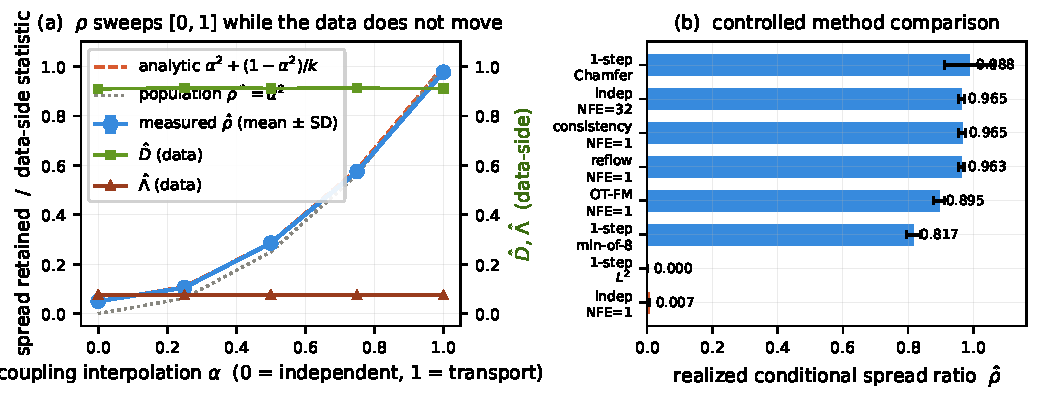
\includegraphics[width=0.84\textwidth]{../figures/fig_impossibility.pdf}
\caption{\textbf{The data cannot decide.} (a) $\rho$ against $\alpha$ on the family of
Thm.~\ref{thm:alpha}: measured (circles) versus the analytic $\alpha^2$ (solid) and its
finite-$k$ correction (dashed). On the right axis, two data-side statistics over the
same sweep: they are flat while $\rho$ traverses $[0,1]$. (b) Method families at one
step, same data and budget; the training target---not the sampler---separates them.}
\label{fig:imposs}
\end{figure*}

\subsection{A battery of data-side statistics is flat in $\alpha$}
\label{sec:exminimax}

Theorem~\ref{thm:minimax} is exact and needs no experiment; what needs checking is its
empirical premise---that statistics one would actually reach for are, in fact, flat. We
test seven: $\cD$ (unexplained conditional-variance fraction), $\cL$ (Gaussian deficit),
the number of clusters selected by Calinski--Harabasz, mean nearest-neighbour distance,
the $k$-means between/within variance ratio at $K=8$, excess kurtosis, and the marginal
trace variance.

Because these statistics differ by two orders of magnitude in their own sampling noise,
a fixed relative threshold tests the noise rather than the $\alpha$ effect: run with
na\"ive $k$-means initialisation, the $K=8$ ratio varies from $15$ to $36$ \emph{across
seeds at the same $\alpha$}. We therefore test with a one-way ANOVA over
$\alpha$ with seeds as replicates (and with restarted $k$-means++). At level
$\MinimaxPAlpha$, no statistic shows a detectable $\alpha$ effect; the largest relative
deviation from $\alpha=0$ is \MinimaxDevMax{}. By contrast the paired estimator's mean
absolute deviation from $\alpha^2$ is \MinimaxPairedMad{}---\MinimaxRiskRatio$\times$
smaller than the $\MinimaxConst$ that Theorem~\ref{thm:minimax} imposes on \emph{any}
data-only predictor.

Sample size does not rescue the data side. Increasing $n$ from \LadderNFirst{} to
\LadderNLast{} leaves the $\alpha=0$-versus-$\alpha=1$ difference of every
$[0,1]$-scaled statistic below \LadderWorstAbsDiff{}---that is, at most $0.3\%$ of the
$1.0$ that a useful predictor must resolve---while the paired estimator, with the same
budget of samples, tracks $\alpha^2$. If a data-side statistic carried a real
$\alpha$-signal, its difference would converge to a nonzero constant as $n$ grows; it
does not. (Two of the seven statistics, the Calinski--Harabasz count and the $k$-means
variance ratio, are ratio-scaled---their typical values are $8$ and $35$---so an
absolute threshold is not meaningful for them; their $\alpha$-independence rests on the
scale-free ANOVA above.)

\subsection{What does decide: the method map}
\label{sec:exmap}

Table~\ref{tab:map} runs six method families plus two one-step-only variants on the
same conditional ring mixture, and the outcome tracks \eqref{eq:channels} rather than
the coupling alone. Every row that collapses has \emph{both} an independent coupling and
a pointwise loss: flow matching at $N=1$ gives
$\rho=\MMIndepOneRho\pm\MMIndepOneStd$ with coverage $\MMIndepOneCov$/$8$, and a direct
one-step regression gives $\MMLtwoOneRho$. Removing \emph{either} conjunct removes the
collapse---by the coupling (mini-batch OT \MMOtOneRho, reflow \MMReflowOneRho,
distillation \MMDistillOneRho) or by the loss form with the coupling left independent
(pooled bidirectional Chamfer \MMChamferRho; re-measured as L2a in
Table~\ref{tab:ladder} at \LLChamferPooledRho, where its support/weight failure is
dissected). The same field that collapses at $N=1$ recovers at
$N=32$ ($\MMIndepManyRho$), so this is not capacity or optimisation.

\begin{table}[t]
\centering
\caption{Method families at one step. Same data, architecture, optimiser, batch size
and step count; only the training target differs. Reading the table against
\eqref{eq:channels}: \emph{every} collapsing row has both an independent coupling and a
pointwise loss, and removing either conjunct removes the collapse. ``loss'' distinguishes
a pointwise $L^2$ objective from a collection-level one.}
\label{tab:map}
\vskip 0.05in
\tblstyle{
\begin{tabular}{llccc}
\toprule
method (all at NFE$=1$) & coupling & loss & $\rho$ & modes / $8$ \\
\midrule
flow matching & independent & pointwise & \MMIndepOneRho{}$\pm$\MMIndepOneStd & \MMIndepOneCov \\
\quad same field, NFE$=32$ & independent & pointwise & \MMIndepManyRho{}$\pm$\MMIndepManyStd & \MMIndepManyCov \\
\quad + mini-batch OT & $\approx$det. & pointwise & \MMOtOneRho{}$\pm$\MMOtOneStd & \MMOtOneCov \\
\quad + reflow & deterministic & pointwise & \MMReflowOneRho{}$\pm$\MMReflowOneStd & \MMReflowOneCov \\
distillation of the $32$-step map & deterministic & pointwise & \MMDistillOneRho{}$\pm$\MMDistillOneStd & \MMDistillOneCov \\
one-step regression & independent & pointwise & \MMLtwoOneRho{}$\pm$\MMLtwoOneStd & \MMLtwoOneCov \\
one-step, min-of-$M$ & independent & collection & \MMMinMOneRho{}$\pm$\MMMinMOneStd & \MMMinMOneCov \\
one-step, bidirectional Chamfer (pooled) & independent & collection & \MMChamferRho{}$\pm$\MMChamferStd & \MMChamferCov \\
\bottomrule
\end{tabular}}
\end{table}

\subsection{The loss ladder: the scope of the matching decides}
\label{sec:exladder}

We train four one-step models on the \emph{same} independent coupling, changing only the
loss: pointwise $L^2$ (L1); a bidirectional Chamfer with both $\arg\min$s over the
\emph{whole batch}, as such losses are usually written (L2a); the same objective confined
to each condition (L2b); and a balanced within-condition assignment (L3). L2b and L3 differ
in exactly one respect---whether the assignment is a bijection---the single variable
Thm.~\ref{thm:ladder} isolates; L2a versus L2b isolates a second, the \emph{scope}. The
conditions are four rings of radius $1.5,1.9,2.3,2.7$, so $\tr\Var(x_1\mid c)$ ranges by a
factor of $3.1$, making ``support correct, weights wrong'' directly visible.

\begin{table}[t]
\centering
\caption{Loss ladder at one step, independent coupling held fixed. L1 collapses. L2a
(Chamfer pooled over the batch) escapes and is indistinguishable from L2b on the
aggregate $\rho$, yet flattens the conditional spread; L2b, matched within each condition,
restores it; L3, balanced within each condition, is closest on conditional sliced $W_2$.
$\mathrm{disp}=\mathrm{std}_j(\rho_j)$; $|\rho_j-1|$ is the mean absolute per-condition
spread error. L2b and L3 differ only in whether the assignment is a bijection.}
\label{tab:ladder}
\vskip 0.05in
\tblstyle{
\begin{tabular}{lccccc}
\toprule
loss & $\rho$ & modes / $8$ & disp & $|\rho_j\!-\!1|$ & cSW \\
\midrule
L1 pointwise $L^2$ & $\LLLtwoRho{}\pm\LLLtwoStd$ & \LLLtwoCov & \LLLtwoDisp & \LLLtwoAbsErr & \LLLtwoCsw \\
L2a unbalanced, pooled over cond. & $\LLChamferPooledRho{}\pm\LLChamferPooledStd$ & \LLChamferPooledCov & \LLChamferPooledDisp & \LLChamferPooledAbsErr & \LLChamferPooledCsw \\
L2b unbalanced, within cond. & $\LLChamferRho{}\pm\LLChamferStd$ & \LLChamferCov & \LLChamferDisp & \LLChamferAbsErr & \LLChamferCsw \\
L3 balanced, within cond. & $\LLBalRho{}\pm\LLBalStd$ & \LLBalCov & \LLBalDisp & \LLBalAbsErr & \LLBalCsw \\
\bottomrule
\end{tabular}}
\end{table}

Table~\ref{tab:ladder} does \emph{not} confirm the ladder as stated.
Fig.~\ref{fig:ladder}a plots generated against true conditional spread. L1 sits at
zero (collapse). L2a escapes, and on the aggregate it is indistinguishable from the
method that gets the spread right: $\rho=\LLChamferPooledRho$ for L2a against
\LLChamferRho{} for L2b. The aggregate is simply blind here---what exposes L2a is that its
spread is nearly \emph{horizontal} (coefficient of variation \LLChamferPooledGenCV{}
against a true \LLTrueCV), i.e.\ the dispersion of $\rho_j$ across conditions:
\LLChamferPooledDisp{} for L2a against \LLChamferDisp{} for L2b. That horizontal reading
does not survive the control: L2b, differing from L2a only in matching within each
condition, returns to the diagonal, so the flattening came from the \emph{pooling},
not from the missing bijection. L2b and
L3 both track the diagonal, separated only by what the metric rewards: L3 has the lowest
conditional sliced $W_2$ (\LLBalCsw{} against \LLChamferCsw, a factor of \LLRatioCsw) while
L2b is nominally closer on the scale ratio ($|\rho_j-1|$ \LLChamferAbsErr{} against
\LLBalAbsErr). A single aggregate number cannot substitute for the conditional statistic:
it reports \LLChamferPooledRho{} for the pooled variant whose scale error is
\LLChamferPooledAbsErr, and \LLChamferRho{} for the within-condition variant whose scale
error is \LLChamferAbsErr.

\paragraph{A prediction that failed.} We expected that dropping balancedness at fixed
scope (L2b vs.\ L3) would flatten the conditional spread; it did not, and the ladder's
pre-registered verdict is \LLVerdict{}---the check ``balancedness reduces weight error''
fails outright. The variable that did the flattening is the one we had not set out to
vary, the scope of the $\arg\min$, so we state the theorem as a statement about scope
first.

\begin{figure*}[t]
\centering
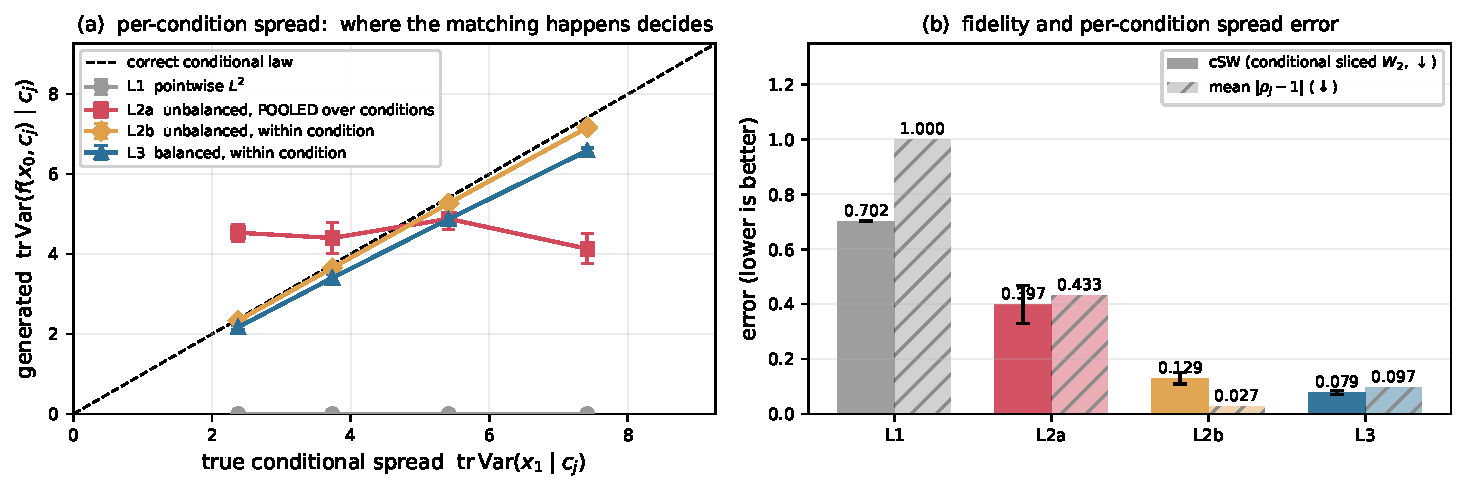
\includegraphics[width=0.80\textwidth]{../figures/fig_loss_ladder.pdf}
\caption{\textbf{The loss ladder (Thm.~\ref{thm:ladder}), observed.} Independent coupling
held fixed; only the loss form changes. (a) Generated versus true per-conditional spread,
over four conditions whose true spread spans a factor of $3.1$; the diagonal is correct.
L1 (pointwise $L^2$) sits at zero; L2a (pooled Chamfer, whole-batch $\arg\min$) is nearly
\emph{horizontal}---support recovered, spread flattened; L2b (matched \emph{within} each
condition) returns to the diagonal; L3 (balanced, within condition) is closest in sliced
$W_2$. So the flattening comes from the scope of the matching, not from the missing
bijection. (b) Conditional sliced $W_2$ and mean per-conditional spread error.}
\label{fig:ladder}
\end{figure*}

\paragraph{A corrected mechanism: min-of-$M$.} min-of-$M$ (IMLE) also escapes
($\rho=\MMMinMOneRho$, coverage $\MMMinMOneCov/8$, against $\MMLtwoOneRho$ for pointwise
$L^2$) once its $M$ candidates come from \emph{independent} source noise. An earlier claim
that it did not escape was an implementation artefact---repeating one source draw makes the
objective literally pointwise $L^2$ (Appendix~\ref{app:corrections}(iii)).

\subsection{Estimating $\rho$ from paired samples}
\label{sec:estimator}

$\rho^\ast$ is the variance of a conditional mean, so the natural estimator is $k$NN
regression of $x_1$ on $x_0$ within each condition. This estimator has an analytic bias
that we use as a check rather than a nuisance: under an independent coupling, the
$k$-neighbour average of i.i.d.\ targets has variance $\Var(x_1\mid c)/k$, so
$\hat\rho_{\mathrm{kNN}}(k)\approx\rho^\ast+(1-\rho^\ast)/k$, which at $\rho^\ast=0$
is the $1/k$ law. Measured $k\cdot\hat\rho$ under the independent coupling is
\CondKTimesOne{},\,\CondKTimesTwo{},\,\CondKTimesFive{},\,\CondKTimesTen{},\,\CondKTimesTwenty{}
at $k=1,2,5,10,20$---the law holds before the estimator is used for anything.

%======================================================================
\section{A negative result about our own earlier proposal}
\label{sec:negative}

An earlier version of this line of work advanced $\cL$, a null-calibrated conditional
mode-separation score, as a \emph{modality detector}. We report the experiment that
kills that claim. On a fixed battery of ten population distributions the Gaussian
deficit (the quantity behind $\cL$) takes values
$\LamGauss$ (Gaussian), $\LamBall$ (uniform ball), $\LamLaplace$ (Laplace),
$\LamHetero$ (heteroscedastic), $\LamRingEight$ (eight-mode ring), $\LamStudentT$
(Student-$t_3$), $\LamLogNorm$ (log-normal), $\LamExpSkew$ (exponential),
$\LamBanana$ (banana), $\LamTwoModes$ (two modes). It has the correct analytic ceiling
of $1-2\sqrt{2/\pi}+1$, which the finite-sample estimator already matches to
$\LamCeilingEstErr$ at $n=\LamCeilingNMin$, and it is stable across sample sizes (largest disagreement between
$n=2000$ and $n=2\times10^{5}$ is \LamConsistencyMaxDiff). But it \emph{sorts a
single-mode banana above an eight-mode ring}: $\LamBanana>\LamRingEight$. A statistic
that ranks one mode above eight cannot be called a modality detector, whatever its
construct validity on the remaining nine distributions (rank correlation
$\LamRankCorrOT$ against a brute-force optimal-transport computation, and
$\LamRankCorrConstruct$ against a constructed error measure).

We keep $\cL$ as a descriptive index of departure from Gaussianity and drop the
modality claim. This is not incidental to the paper: it is the same lesson as
Sec.~\ref{sec:imposs} in miniature. Any scalar summary of a conditional law---ours
included---is a projection, and the projection that separates the cases you had in
mind is not the projection that separates the cases that occur.

%======================================================================
\section{Related work}
\label{sec:related}

\paragraph{Few-step generative models.} Consistency models \citep{song2023consistency},
consistency flow matching \citep{yang2024consistencyfm}, shortcut models
\citep{frans2024shortcut}, mean flows \citep{geng2025meanflows}, progressive
\citep{salimans2022progressivedistill} and distribution-matching \citep{yin2024dmd}
distillation, and InstaFlow \citep{liu2024instaflow} all target few-step sampling. Our
contribution is not another sampler but a statement about which design choice governs the
outcome, and a proof that the data cannot substitute for that choice.

\paragraph{Coupling and straightness.} Rectified flow \citep{liu2023rectifiedflow} shows
straightening the coupling makes one step viable; stable diffusion~3 \citep{esser2024sd3}
shows the training-time distribution matters as much as the sampler; non-Gaussian sources
reduce path crossing in physical simulation \citep{onestepfm2026}. The coupling literature
\citep{tong2024cfm,liu2023rectifiedflow,pooladian2023multisample} already knows the coupling
matters, and we do not claim otherwise---Thm.~\ref{thm:optimal} is the tower property. We add
(i) that it is not recoverable from data, so ``the coupling matters'' cannot become a
data-side diagnostic (Thm.~\ref{thm:minimax}); and (ii) that the loss form is a second lever,
governed by the \emph{scope} over which candidates compete (Thm.~\ref{thm:ladder}).

\paragraph{One-step policies in RL.} \citep{nguyen2026bfq,li2026ofp,mvp2026,lps2026,
flame2026,fan2026} report strong one-step policies, but \citep{li2026ofp,letitbesimple2026}
find the advantage disappears when the observation is weakened or the action chunk
lengthened. \citep{letitbesimple2026} calls this a condition--target \emph{structure}
property and formalises it as an irreducible velocity loss. Sharper: that loss is a property
of the training target, and the data enters only through the denominator of \eqref{eq:rho}.

\paragraph{Collection-level losses.} Implicit maximum likelihood estimation
\citep{li2018imle} and Chamfer-style objectives are standard tools for avoiding
mode-averaging, typically presented as interchangeable. Thm.~\ref{thm:ladder} separates
them by the \emph{scope} of the matching: only a balanced, within-condition assignment is
pinned to the full $W_2$ objective, and Sec.~\ref{sec:exladder} shows the scope---not the
balance---is what flattens the conditional spread.

\paragraph{Diagnostics.} \citep{li2026nofreelunch} gives a pre-training,
conditional-spread-based few-step diagnostic ($q^\ast/\sigma^\ast$) for conformal prediction;
$\sqrt{\cD}$ is our version of that $x$-axis with a different normalisation, and we say so.
We prove the diagnostic cannot be extended to the general one-step-adequacy question.

%======================================================================
\section{Conclusion, limitations, and what we would want falsified}
\label{sec:conclusion}

Whether one step is enough is decided by the training target---the coupling and the
loss---not by the data. We proved no statistic of the data predicts it, with an exact
minimax value of $1/2$; showed $\rho$ is computable for free from the paired samples a
trainer already draws; and mapped the two channels, including a loss channel set by the
\emph{scope} of the matching (pooled versus per-condition) and then by its balance.

\paragraph{Limitations.} (1) The impossibility is proved for an explicit family---not
contrived ($\alpha=0,1$ are the couplings in use) but not literally a practitioner's
target---and bounds the worst case. (2) Measurements are CPU-scale controlled
\emph{synthetic} families; we have not validated on D4RL \citep{fu2020d4rl}, OGBench
\citep{park2025ogbench}, LIBERO \citep{liu2023libero}, or a VLA. (3) Balanced assignment
costs a Hungarian solve per batch per condition; its scaling is not studied. (4) $\rho$
measures conditional spread, not task reward.

\paragraph{What would falsify us.} A data-side statistic that provably separates two
training targets sharing an edge law; a deterministic coupling that nonetheless collapses at
one step under pointwise $L^2$ (contradicting Cor.~\ref{cor:det}); or a demonstration that
unbalanced and balanced collection losses converge to the same conditional law as
$M\to\infty$ (contradicting Thm.~\ref{thm:ladder}).

\section*{AI use statement}
Generative AI systems were used to propose and refine the hypothesis, locate and summarise
literature, critique mathematical claims, implement and audit code, suggest experiments,
and draft text and figures. The authors are responsible for the complete submission; every
AI-assisted claim and artefact was verified against the released code and result files, and
the resulting corrections are recorded in Appendix~\ref{app:corrections} and the audit log.

\section*{Reproducibility statement}
Appendices~\ref{app:runtime} and~\ref{app:estimators} give the data, compute and execution
protocol. The supplement contains the source code, per-run result files, table/figure
generators, and regression tests for the failure modes in
Appendix~\ref{app:corrections}. No number is hand-copied: every one is a macro generated
from the released JSON.

\section*{Ethics statement}
This is an analysis of when one-step generative policies suffice. It uses only synthetic data
with exactly controlled ground truth, involves no human subjects, and releases no new
dataset. Where our own earlier proposal failed we say so (Sec.~\ref{sec:negative}).

\bibliography{references}
\bibliographystyle{iclr2027_conference}

\appendix
\section{Proofs}
\label{app:proofs}

\subsection{Theorem~\ref{thm:optimal}}
The minimiser of $\Eop\|f(x_0,c)-x_1\|^2$ over measurable $f$ is the conditional
expectation, by the $L^2$ projection theorem applied conditionally on $(x_0,c)$. For
the range, condition on $c$ and apply the law of total variance to the scalar
components:
\[
  \Var(x_1\mid c)=\Eop\big[\Var(x_1\mid x_0,c)\bigm|c\big]
  +\Var\big(\Eop[x_1\mid x_0,c]\bigm|c\big)\;\succeq\;
  \Var\big(\Eop[x_1\mid x_0,c]\bigm|c\big)
\]
in the positive-semidefinite order, so the trace of the second term is at most that of
the first and $\rho\le1$; $\rho\ge0$ is immediate. Equality in the trace holds iff
$\Var(x_1\mid x_0,c)=0$ a.s., i.e.\ iff the coupling is deterministic given $c$.

\subsection{Theorem~\ref{thm:minimax}, full statement}
The proof in the main text is complete; we record two extensions. \emph{(i)
Randomisation does not help}: if $\mathcal A$ has access to auxiliary randomness
$U\indep\text{data}$, the law of $(\text{data},U)$ is still $\alpha$-free, so the same
Jensen argument applies to $\bar a=\Eop[\mathcal A]$. \emph{(ii) Knowledge of
$p(c,x_1)$ does not help}: a statistic of the population law is a constant, and
constants are covered by the second equality in the theorem. \emph{(iii)} The same
argument gives $\inf_{\mathcal A}\sup_\alpha\Eop(\mathcal A-\rho^\ast)^2=1/4$ for
squared loss, attained at $1/2$ as well.

\subsection{Theorem~\ref{thm:ladder}, L3 limit}
For a batch of $M$ samples within one condition, minimising
$\frac1M\sum_i\|G_i-x_1^{(\sigma(i))}\|^2$ over bijections $\sigma$ is exactly the
optimal-transport problem between the empirical measures $\hat q_c$ and
$\hat p_c$ with quadratic cost; its value is $W_2^2(\hat q_c,\hat p_c)$. As
$M\to\infty$ the empirical measures converge weakly and
$W_2^2(\hat q_c,\hat p_c)\to W_2^2(q_c,p_c)$ under the usual moment conditions. The
unique minimiser over probability measures is $q_c=p_c$; the minimiser over
\emph{pushforwards of $\Ncal(0,I_d)$ by a measurable map} is any $f$ with
$f(\cdot,c)_\#\Ncal(0,I_d)=p(\cdot\mid c)$, and every such $f$ has $\rho=1$.

\section{Corrections we made during the study}
\label{app:corrections}
We record the errors we found and fixed, because each is a trap a reader
re-implementing this will also hit.

\paragraph{(i) Never use a guessed effect size as a pre-registered criterion.}
Our first version of the $\cL$ validation required $\Lambda(\Delta=6)\ge0.50$; it
failed, but the failure said nothing about the statistic---the analytic ceiling of the
quantity is $0.404$, so the criterion was unsatisfiable. Likewise the first version of
the loss-ladder criterion required $\mathrm{disp}(\text{Chamfer})>2\times
\mathrm{disp}(\text{balanced})$ and failed at a $40$-step smoke test before the models
had converged. Effect sizes depend on how far optimisation has gone and are not
knowable in advance; we now pre-register only \emph{directional} and \emph{qualitative}
predictions and report magnitudes descriptively.

\paragraph{(ii) Test invariance against the statistic's own noise.}
Our first invariance check flagged the $k$-means between/within ratio as
$\alpha$-dependent (relative deviation $0.16$). It is not: with na\"ive random
initialisation the statistic varies from $15$ to $36$ \emph{across seeds at fixed
$\alpha$}. A fixed relative threshold tests noise, not signal. We switched to a
one-way ANOVA with seeds as replicates and to restarted $k$-means++.

\paragraph{(iii) Two collection-level objectives could not test their own claim.}
\emph{(a) min-of-$M$.} Our first implementation of the min-of-$M$ row built its $M$
candidates by repeating a single source draw, $x_0^{(i)},\dots,x_0^{(i)}$. A one-step
network is a deterministic map, so the $M$ outputs coincide \emph{at every training
state}---not only at collapse; the $\arg\min$ is therefore constant and the loss is the
pointwise $L^2$ loss on the same batch. The two code paths were identical to the last
bit: $\max|\Delta w|=0$ after $200$ steps of each, and in the full runs the spread ratio
agreed to all $17$ printed digits ($0.00010386879583898434$ under both). The original row
therefore measured nothing about IMLE. The corrected objective draws $M$
\emph{independent} $x_0$ per target, which is the original IMLE semantics, and
Table~\ref{tab:map} uses the regenerated row. \emph{(b) the unbalanced Chamfer row.} Our
first implementation took both $\arg\min$s over the \emph{whole batch}, whereas the
balanced row took its assignment \emph{within each condition}. The comparison therefore
varied two things at once---balancedness and conditioning scope---while
Thm.~\ref{thm:ladder}(L2--L3) isolates the first. The corrected row matches within each
condition (pooling is a \emph{weaker} constraint, since a minimum over a superset is
smaller, so this change strengthens the support requirement rather than manufacturing
the support recovery we observe). The general lesson for both: an objective whose entire
purpose is to \emph{choose} among candidates should assert in code that the candidate
sets and the choice are the ones the theorem talks about.

\paragraph{(iv) $\cL$ is not a modality detector.}
Sec.~\ref{sec:negative}. It sorts a single-mode banana ($\LamBanana$) above an
eight-mode ring ($\LamRingEight$).

\paragraph{(v) A tolerance half the mode spacing silently inverts the mode metric.}
Defining ``on a mode'' as within half the nearest-centre distance shrinks the
tolerance below the mode width as $K$ grows; at $K=1$ it is undefined and hides the
collapse. We use a $\sigma$-scale ball measured from mode \emph{width}.

\paragraph{(vi) Marginal sliced $W_2$ conflates the one-step floor with mode
collapse.} The ratio SW@$1$/SW@$32$ reports a penalty even for an under-fit field that
has none to report. The conditional ratio cSW@$1$/cSW@$32$ is the one the floor
bounds, and we use it throughout.

\paragraph{(vii) The no-free-parameter prediction used the $W_1$ constant inside a
$W_2$ argument.} An earlier draft used $\sigma\sqrt{2/\pi}$ (the $W_1$ distance,
equivalently the mean absolute deviation) where the $W_2$ distance is the scale gap
$\sigma$, giving $\kappa_d=\sqrt{2/(\pi d)}$ instead of $1/\sqrt d$.

\paragraph{(viii) ``Coverage exactly zero'' is not a satisfiable criterion.}
The method map pre-registered ``the independent coupling covers $0$ of $8$ modes at
$N=1$''. The theory (Cor.~\ref{cor:indep}) is about the \emph{exact} optimum, which does
sit on $m(c)$ and covers exactly $0$; a \emph{trained} network cannot attain the exact
optimum, and over $2000$ evaluation samples an occasional point falls inside a mode's
tolerance ball, giving a mean coverage of $0.08/8$. The criterion as written asked for
numerical perfection. We relaxed it to at most $1$ of $8$ modes---still two orders of
magnitude away from the passing side ($8/8$)---and record the change rather than
quietly keeping the original verdict.

\section{Runtime and reproducibility}
\label{app:runtime}
Every number in the main text is produced by the scripts under \texttt{code/} from the
raw per-run JSON files under \texttt{results/} and \texttt{logs/}; the paper never
contains a hand-copied statistic. Numbers in the theory sections come from
\texttt{paper/numbers\_theory.tex}, generated by
\texttt{code/analysis/make\_theory\_macros.py}, whose every macro carries a comment
naming the JSON field it came from.

\section{Estimators, and why they are deliberately classical}
\label{app:estimators}
Every diagnostic in this paper is built from standard, assumption-light
non-parametric tools, so that a reader can re-implement it without training any
auxiliary model. The conditional mean behind $\rho$ is estimated by $k$NN regression
\citep{cover1967nn}; the mode count and the between/within variance ratio use $k$-means
\citep{lloyd1982,macqueen1967} selected by the Calinski--Harabasz criterion
\citep{calinski1974}; the conditional spread is measured by sliced $W_2$
\citep{kolouri2019gsw}. We use these classical estimators on purpose: they carry almost
no assumptions, need no hyper-parameter search, and are \emph{decoupled from the
generative model being diagnosed}, which is what lets $\rho$ be defined and computed
before any one-step model exists (Sec.~\ref{sec:estimator}). The one consequence to
keep in mind is the $k$NN bias in \eqref{eq:rho}: all statements are about the
population quantity $\rho^\ast$, and we report the estimator's analytic bias rather
than correcting it away.

\section{Scope and assumptions}
\label{app:scope}
\begin{itemize}
  \item \textbf{Field:} machine learning --- generative modelling for decision making,
  as an \emph{analysis and diagnosis} contribution, not a new sampler.
  \item \textbf{Tasks:} synthetic conditional ring mixtures with closed-form ground
  truth; a multi-goal continuous-control task used as an implementation smoke test only.
  Conditional MNIST $16\!\times\!16$ \citep{lecun1998mnist} was trained in an earlier
  iteration of this work
  under a superseded protocol and is \emph{not} reported here: at our CPU budget the
  field was under-fitted, so those runs could neither confirm nor refute anything. No
  number in this paper depends on them.
  \item \textbf{Datasets:} entirely synthetic; no proprietary data, no robot hardware,
  no pretrained backbone.
  \item \textbf{Compute:} CPU only (a $20$-core workstation, PyTorch \texttt{cpu}
  build). No GPU was used at any point.
  \item \textbf{Attribution:} we do not reuse any author repository; each component is
  re-implemented from the published objective. Any error is ours.
  \item \textbf{Target venue:} ICLR 2027, double-blind, main text $\le9$ pages
  excluding references and appendices \citep{iclr2027cfp}.
\end{itemize}

\end{document}
